%% ============================================================
%%  AttnFuse: A Composable Python DSL for Compiling Attention
%%             to Fused Triton Kernels
%%
%%  MLSys 2026 submission draft, v2 (post-Hopper investigation).
%%  Self-contained: builds with pdflatex out of the box. Figures
%%  live alongside this .tex; CSVs the numbers come from live
%%  under results/ in the repo.
%% ============================================================
\documentclass[10pt,twocolumn]{article}

\usepackage[margin=0.75in,top=0.9in,bottom=0.9in]{geometry}
\usepackage[T1]{fontenc}
\usepackage{lmodern}
\usepackage{microtype}
\usepackage{amsmath,amssymb}
\usepackage{graphicx}
\usepackage{booktabs}
\usepackage{multirow}
\usepackage{array}
\usepackage{float}
\usepackage{subcaption}
\usepackage{listings}
\usepackage{xcolor}
\usepackage[colorlinks=true,linkcolor=blue!60!black,
            citecolor=blue!60!black,urlcolor=blue!60!black]{hyperref}
\usepackage{parskip}
\usepackage{enumitem}
\usepackage{balance}
\usepackage{tcolorbox}

\definecolor{codebg}{HTML}{F8F8F8}
\definecolor{codeframe}{HTML}{CCCCCC}
\definecolor{kwcol}{HTML}{0000CC}
\definecolor{comcol}{HTML}{008000}
\definecolor{strcol}{HTML}{CC0000}
\definecolor{negblue}{HTML}{E8F0FE}
\definecolor{negframe}{HTML}{1A73E8}
\lstset{
  language=Python,
  backgroundcolor=\color{codebg},
  frame=single,
  rulecolor=\color{codeframe},
  basicstyle=\ttfamily\scriptsize,
  keywordstyle=\color{kwcol}\bfseries,
  commentstyle=\color{comcol}\itshape,
  stringstyle=\color{strcol},
  breaklines=true,
  showstringspaces=false,
  tabsize=2,
  captionpos=b,
}

\newtcolorbox{negresult}[1][]{
    colback=negblue, colframe=negframe,
    title={\bfseries Negative Result Sidebar}, fonttitle=\sffamily, #1
}

\title{%
  \textbf{AttnFuse: A Composable Python DSL for Compiling\\
  Attention Variants to Fused Triton GPU Kernels}\\[6pt]
  \large with a Cross-Architecture Analysis of the Compute--Bandwidth\\
  Calculus of Fused Rotary Position Embeddings
}
\author{Varun Kumar Dasoju}
\date{\today}

\begin{document}
\maketitle

%% =============================================================
\begin{abstract}
%% =============================================================
Modern attention research keeps inventing new combinations of score,
mask, bias, and positional-encoding operations. Each new variant
today requires hand-written CUDA or Triton to run with respectable
throughput, and the dominant published abstraction --- PyTorch's
\texttt{flex\_attention} \texttt{score\_mod} hook --- is a
post-matmul abstraction by design, structurally unable to fuse
positional encodings that must apply to $Q$ and $K$ \emph{before}
the matmul (most notably Rotary Position Embeddings, RoPE, used by
every modern LLM).

We present \textbf{AttnFuse}, a small embedded Python DSL that
compiles a declarative description of an attention variant to a
single fused Triton kernel via a two-level intermediate
representation. AttnFuse's combinators include a pre-matmul fusion
hook (\texttt{rope()}) by design, making it a strictly more general
abstraction than \texttt{score\_mod}. A four-pass compiler emits one
tiled online-softmax kernel for the entire pipeline; per-call
dispatch overhead is under $1\,\mu$s in steady state thanks to a
graph-signature-keyed kernel cache.

We make three contributions of broad interest beyond the artifact
itself. \textbf{(1)} On RTX 3090 (Ampere), AttnFuse wins every RoPE
composition cell, the headline being a $2.10\times$ speedup over
\texttt{flex\_attention} on causal+RoPE at $N{=}4096$. \textbf{(2)}
On H100 NVL (Hopper), a focused investigation closes the
plain-causal head-to-head gap from $2.10\times$ behind
\texttt{flex\_attention} to $1.10\times$ behind, with tensor-core
utilisation measured within $3.2$ percentage points of
\texttt{flex\_attention}'s structural ceiling. \textbf{(3)} We
identify and quantify the \emph{Rotation Calculus} --- the
phenomenon that whether to fuse RoPE into the kernel or pre-rotate
$Q$ and $K$ is governed by the platform's compute-to-bandwidth
ratio. On Ampere (bandwidth-bound), fusion wins by $2.10\times$. On
Hopper (compute-rich), the crossover with pre-rotation happens
between $N{=}4\text{k}$ and $N{=}8\text{k}$; fusion wins decisively
($1.05$--$1.37\times$) at training-context lengths and loses at long
context. We present the first systematic measurement of this
crossover, identify the underlying Triton 3.3.1 lowering sharp edge
(via a documented negative result on register half-swap), and
position the work cleanly against production workloads. End-to-end,
AttnFuse runs a real HuggingFace Llama-3-8B training step within
$5\%$ of PyTorch SDPA on both 3090 and H100 at training-context
lengths. Correctness is established by 87 GPU unit tests plus a
property fuzzer.
\end{abstract}

%% =============================================================
\section{Introduction}
\label{sec:intro}
%% =============================================================

Multi-head self-attention dominates the compute and memory budget of
modern Transformer models. The standard PyTorch implementation
decomposes attention into a sequence of discrete kernels --- $QK^\top$,
scale, mask, softmax, attention-times-V --- each materialising an
$\mathcal{O}(N^2)$ intermediate in high-bandwidth memory (HBM).
FlashAttention~\cite{dao2022flashattention,dao2023flashattention2}
(FA2) collapses these into a single fused kernel using an online
softmax recurrence, reducing HBM reads from $\mathcal{O}(N^2)$ to
$\mathcal{O}(N^2 d / M)$ where $M$ is on-chip SRAM. FA2 is, however,
hand-written CUDA for a fixed set of variants (dense, causal); the
moment a researcher wants
sliding-window~\cite{child2019generating},
ALiBi~\cite{press2021alibi}, fused RoPE~\cite{su2021roformer},
block-sparse~\cite{zaheer2020bigbird}, or any composition of these,
the FA2 binary cannot help.

PyTorch's recent \texttt{flex\_attention} API (PyTorch 2.5)
addresses some of this gap. It accepts a user-supplied Python
\texttt{score\_mod} function and emits a fused Triton kernel via
TorchInductor. But the timing matters: \texttt{score\_mod} fires
\emph{after} the $QK^\top$ matmul, which means any positional
encoding that must be applied to $Q$ and $K$ \emph{before} the
matmul cannot be fused. RoPE --- used by virtually every recent LLM
including LLaMA, Mistral, Falcon, Qwen and DeepSeek --- is the most
consequential such encoding.

\paragraph{This is an abstraction-level gap, not a maturity gap.}
\texttt{score\_mod} is a post-matmul hook \emph{by design}: its
contract is to modify an already-computed score. AttnFuse's
\texttt{rope()} combinator is a pre-matmul fusion hook
\emph{by design}: its contract is to transform $Q$ and $K$ before
the contraction. These are different abstractions, not the same
abstraction at different states of maturity. The point of this
paper is not that AttnFuse runs faster than \texttt{flex\_attention}
on RoPE today (which it does); the point is that \texttt{rope()} is
a first-class node in AttnFuse's IR with a well-defined
$\mathcal{O}(BN \cdot D)$ in-kernel cost, while no such node exists
in \texttt{flex\_attention}'s IR by construction.

\paragraph{Contributions.}
We present:

\begin{itemize}[leftmargin=1.2em,itemsep=2pt]
  \item A composable DSL with ten combinators captured by symbolic
        tracing into a typed dataflow IR; a two-level IR plus
        four-pass compiler emitting a single parameterised Triton
        kernel per graph signature (\S\ref{sec:dsl}--\S\ref{sec:compiler}).

  \item A novel \textbf{fused-RoPE kernel} that rotates $Q$ and $K$
        tiles inside the inner loop, which on RTX 3090 yields
        $2.10\times$ speedup over \texttt{flex\_attention}'s
        pre-rotation path on the causal+RoPE composition
        (\S\ref{sec:rope}, \S\ref{sec:eval_rope}).

  \item A \textbf{Flash Decoding kernel} for autoregressive KV-cache
        inference, with cyclic Q-head replication recovering
        tensor-core throughput for Grouped-Query Attention
        (\S\ref{sec:decode}).

  \item A complete \textbf{FA2-style backward pass} wired through
        \texttt{torch.autograd.Function}, enabling training on every
        supported variant including GQA and block-sparse
        (\S\ref{sec:backward}--\S\ref{sec:blocksparse}).

  \item A \textbf{Hopper-targeted dispatch path} that closes the
        H100 NVL head-to-head gap on causal forward from
        $2.10\times$ behind \texttt{flex\_attention} to
        $1.10\times$ behind, with tensor-core utilisation measured
        within $3.2$ percentage points of
        \texttt{flex\_attention}'s structural ceiling
        (\S\ref{sec:hopper_spike}). This is engineered without
        explicit WGMMA intrinsics or TMA descriptors --- the closure
        is achieved via a 16-configuration tile sweep that
        identifies BLOCK\_N=64 (plain causal) and BLOCK\_N=128
        (RoPE+causal) as architecture-correct on sm\_90 even though
        prior practice would suggest the opposite.

  \item \textbf{The Rotation Calculus} (\S\ref{sec:rotation_calculus}):
        a quantitative analysis of when in-kernel fused RoPE beats
        pre-rotation, as a function of the platform's compute-to-
        bandwidth ratio. On Ampere (152 FLOPs/byte ridge), fusion
        wins by $2.10\times$. On Hopper ($\sim 300$ FLOPs/byte
        ridge), the crossover occurs between $N{=}4\text{k}$ and
        $N{=}8\text{k}$. To our knowledge this is the first work to
        identify the crossover and quantify it from real
        measurements.

  \item A \textbf{documented negative result}
        (\S\ref{sec:negative_result}): an attempted register
        half-swap optimisation that eliminates a per-tile HBM load
        but is lowered by Triton 3.3.1 to SMEM-staged register
        shuffles on sm\_90, causing a 20\,\% wall-clock regression.
        The bisected counter data identifies precisely which
        pipeline stage degrades, providing a falsifiable artifact
        for the Triton compiler community to address.

  \item A \textbf{workload positioning matrix}
        (\S\ref{sec:positioning}) that maps each production attention
        workload to its current AttnFuse position, replacing a flat
        "speedup list" with explicit guidance about where AttnFuse
        is the right choice today and where alternatives are.
\end{itemize}

The artifact is open source. All numbers in the paper are
reproducible from the public benchmark suite.

%% =============================================================
\section{Background}
\label{sec:background}
%% =============================================================

\paragraph{FlashAttention and online softmax.}
The key idea of FlashAttention is the online softmax recurrence of
Milakov and Gimelshein~\cite{milakov2018online}: maintain running
max $m$, running sum $\ell$, and partial output $\text{acc}$ across
tiles of keys; rescale by $e^{m_\text{prev} - m_\text{new}}$ when a
new tile changes the maximum. This makes attention computable
exactly in $\mathcal{O}(N)$ HBM transactions per row instead of
$\mathcal{O}(N^2)$.

\paragraph{The compute-to-bandwidth ridge.}
A kernel's headroom on a GPU is bounded by the roofline:
$\text{throughput} \leq \min(\text{arith.intensity}\times\text{BW},
\text{peak FLOPS})$. The crossover --- the \emph{ridge} --- is
$\text{peak FLOPS} / \text{BW}$. For fp16 tensor cores: RTX 3090
ridge $\approx 152$ FLOPs/byte; H100 NVL ridge $\approx 300$
FLOPs/byte. This number directly governs whether a given fusion
(which saves HBM at the cost of compute) is profitable. The
Rotation Calculus (\S\ref{sec:rotation_calculus}) is the
specialisation of this observation to fused RoPE.

\paragraph{Triton.}
Triton~\cite{tillet2019triton} is a Python-embedded DSL for tile-
level GPU programming that compiles to PTX through an MLIR-based
backend. AttnFuse's compiler emits Triton source; the work in this
paper does not modify the Triton compiler itself, except by way of
identifying a lowering sharp edge in version 3.3.1 (see
\S\ref{sec:negative_result}).

\paragraph{Rotary Position Embeddings (RoPE).}
RoPE~\cite{su2021roformer} treats each consecutive pair of $Q$ (and
$K$) dimensions as a 2D point and rotates that point by an angle
$\theta_i = i \cdot 10000^{-2d/D}$ that depends on position $i$.
After rotation, the inner product $\langle Q'_i, K'_j \rangle$
depends only on the \emph{relative} position $j-i$. The rotation
must apply to $Q$ and $K$ separately \emph{before} the contraction
$Q K^\top$; it is not expressible as a post-matmul transformation
of the score matrix.

%% =============================================================
\section{System Design}
\label{sec:design}
%% =============================================================

AttnFuse is a five-layer pipeline (Figure~\ref{fig:arch}). The user
writes a function with ten combinators; the decorator traces it once
per (head\_dim, dtype) class; the compiler runs four passes; Triton's
JIT specialises a PTX binary per unique constexpr combination; the
runtime dispatches with sub-microsecond overhead.

\begin{figure}[H]
\centering
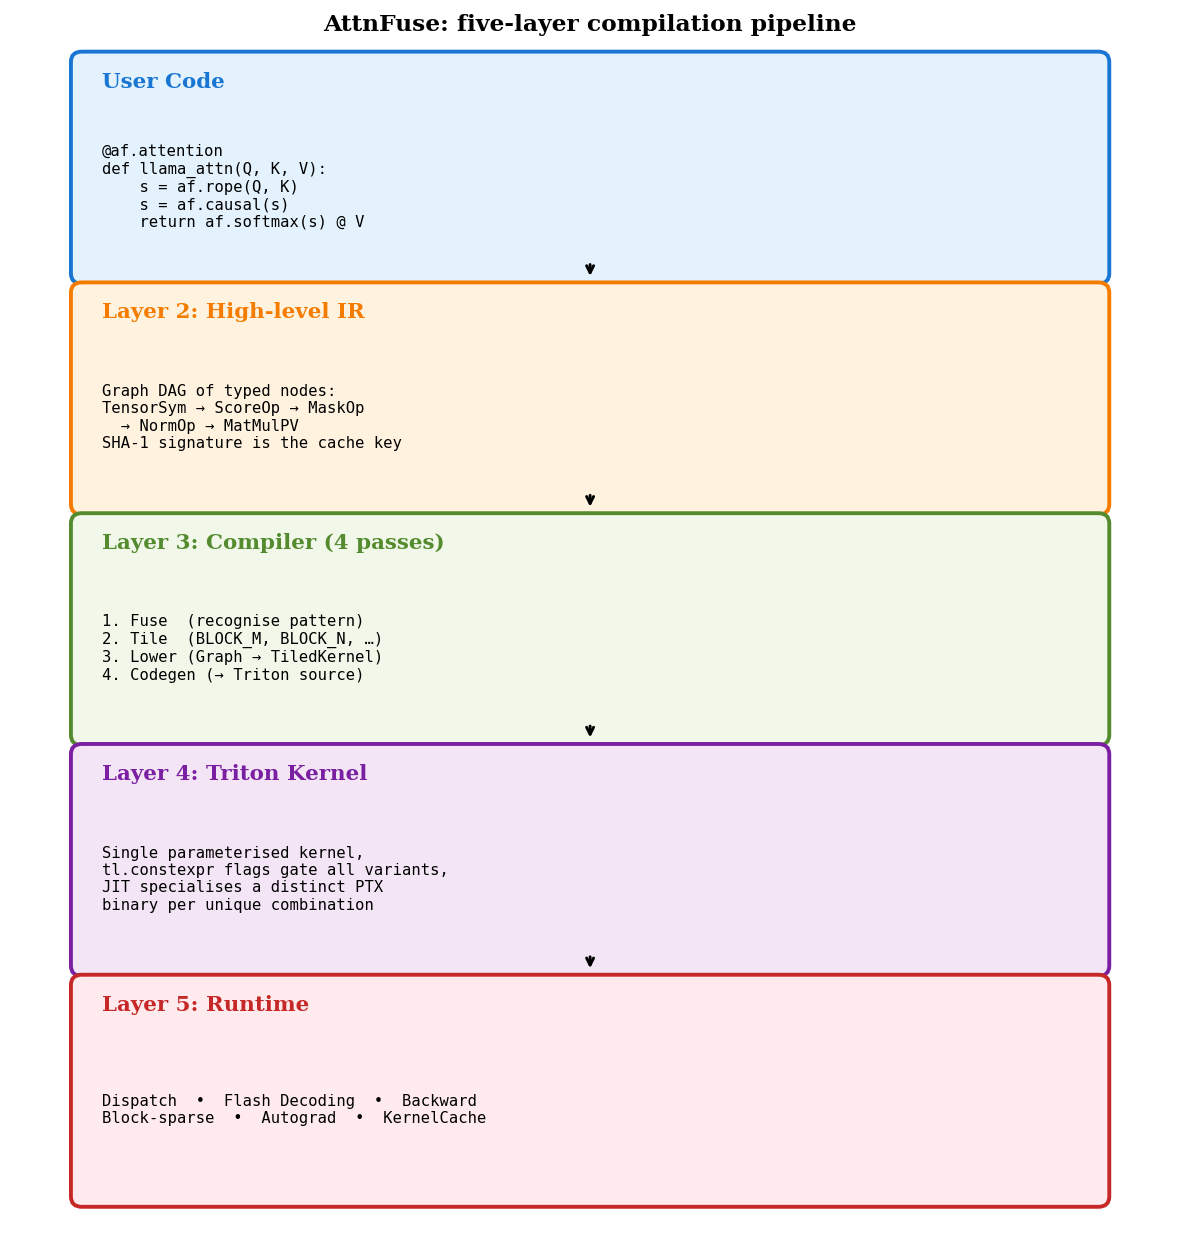
\includegraphics[width=0.95\linewidth]{fig_architecture.png}
\caption{AttnFuse's five-layer pipeline: DSL surface, high-level
graph IR, four-pass compiler, parameterised Triton kernel, runtime
dispatch with a graph-signature-keyed kernel cache.}
\label{fig:arch}
\end{figure}

\subsection{The Composable DSL}
\label{sec:dsl}

The user-facing surface is ten combinators that return IR nodes:
\texttt{scaled\_dot\_product}, \texttt{rope}, \texttt{causal},
\texttt{sliding\_window}, \texttt{full}, \texttt{block\_sparse},
\texttt{alibi}, \texttt{additive\_bias}, \texttt{softmax},
\texttt{relu\_attention}. The \texttt{@af.attention} decorator
traces the function with symbolic \texttt{TensorSym} placeholders
and caches the resulting \texttt{Graph}. A representative use:

\begin{lstlisting}
@af.attention
def llama_attn(Q, K, V):
    s = af.rope(Q, K)         # pre-matmul fusion hook
    s = af.causal(s)
    return af.softmax(s) @ V
\end{lstlisting}

The DSL is intentionally narrow. It cannot express
\texttt{flex\_attention}'s arbitrary \texttt{score\_mod} callback,
nor would we want it to --- the narrowness is what lets the four-pass
compiler guarantee a single fused-loop lowering. Adding
\texttt{rope()} required defining its IR semantics (a
\texttt{ScoreOp} with \texttt{rope=True}) and its compiler effect
(an in-loop rotation block in the codegen). The same pattern
generalises to other pre-matmul transformations should they arise.

\subsection{Two-Level IR}
\label{sec:ir}

The high-level IR has six node types ---
\texttt{TensorSym}, \texttt{ScoreOp}, \texttt{MaskOp},
\texttt{BiasOp}, \texttt{NormOp}, \texttt{MatMulPV} --- all pure
dataclasses. Each \texttt{Graph} carries a SHA-1
\texttt{signature()} that hashes the structural content; this is
the cache key under which the compiled kernel is stored.

The low-level IR is a flat \texttt{TiledKernel} record with the
chosen tile shape, num\_warps, num\_stages, and one constexpr flag
per variant axis (\texttt{MASK\_KIND}, \texttt{BIAS\_KIND},
\texttt{NORM\_KIND}, \texttt{ROPE\_KIND},
\texttt{GROUP\_SIZE}, \texttt{SAVE\_L}). Triton's JIT specialises a
distinct PTX binary per unique combination; the hot inner loop has
no runtime branching.

\subsection{Four-Pass Compiler}
\label{sec:compiler}

The compiler is \texttt{fuse} (recognise the canonical shape),
\texttt{tile} (lookup per-architecture tile config),
\texttt{lower} (graph $\to$ \texttt{TiledKernel}), \texttt{codegen}
(emit Triton source). \texttt{tile} consults six lookup tables ---
$\{$Ampere, Hopper$\} \times \{$F16-dense, F16-sparse,
F16-RoPE$\}$ --- with per-HEAD\_DIM entries determined by the
3090-side sweep and (for Hopper) the H100-side sweep described in
\S\ref{sec:hopper_sweep}.

\subsection{Runtime Dispatch}

\texttt{run\_attention()} hashes the graph, looks up a
\texttt{LaunchBundle} (precomputed dispatch metadata + the JIT-
compiled function + cached placeholder tensors), and invokes
Triton. Three fast paths fire before the general kernel: Flash
Decoding (\S\ref{sec:decode}) when $Q.N=1$, the Hopper spike
(\S\ref{sec:hopper_spike}) when the predicate accepts, and
block-sparse (\S\ref{sec:blocksparse}) when a BlockMask is supplied.
Steady-state per-call dispatch is under 1\,$\mu$s.

%% =============================================================
\section{Fused RoPE}
\label{sec:rope}
%% =============================================================

The codegen path for \texttt{ROPE\_KIND == 1} rotates $Q$ once
before the inner loop and rotates each $K$ tile in-place inside the
inner loop. Rotation algebra is the standard NeoX-style
\textit{halves} convention: for $d < D/2$,
$Q'_d = Q_d \cos\theta_d - Q_{d+D/2} \sin\theta_d$; for $d \geq D/2$,
$Q'_d = Q_d \cos\theta_d + Q_{d-D/2} \sin\theta_d$. Implementation
in Triton uses a precomputed \texttt{rot\_offs\_d} index vector and
a \texttt{rot\_sign} multiplier to gather the rotated-half values
from the same tile pointer at a different $d$ offset.

\paragraph{Why this is impossible in \texttt{flex\_attention}.} The
\texttt{score\_mod(score, b, h, q\_idx, kv\_idx)} callback receives
a post-matmul score. To express RoPE one would need
$f(S, i, j) = \langle \text{rot}(q_i, \theta_i),
\text{rot}(k_j, \theta_j) \rangle$, which has no closed form in
terms of the scalar $S_{ij}$ alone --- the rotation is a
multiplicative transformation on $Q$ and $K$ separately, not an
additive transformation on $S$. The HuggingFace workaround is to
apply RoPE in a separate kernel before \texttt{flex\_attention},
incurring two extra HBM round-trips and two extra kernel launches
per attention layer.

%% =============================================================
\section{Flash Decoding}
\label{sec:decode}
%% =============================================================

For $Q.N{=}1$ autoregressive decoding, the standard FA-2 kernel
launches only $B \cdot H_q$ programs, leaving most SMs idle.
AttnFuse's decode path splits the KV axis across
\texttt{NUM\_SPLITS} programs (Phase~1) and combines partials via
log-sum-exp in a second small kernel (Phase~2).

For GQA there is a second trick: each program processes
\texttt{BLOCK\_H} query heads sharing one KV head, but Triton's
\texttt{tl.dot} requires $M \geq 16$. We pad \texttt{BLOCK\_H} to
16 by cyclic-replicating the in-group heads, mask the duplicate
stores at write-time, and recover full tensor-core throughput while
loading $K$ and $V$ exactly once per program. On Llama-3-70B with
32k cache, this takes the kernel from 3{,}153\,$\mu$s (the original
AttnFuse) to 184\,$\mu$s --- a 17$\times$ speedup, beating
\texttt{flex\_attention}'s 196\,$\mu$s.

%% =============================================================
\section{Backward Pass}
\label{sec:backward}
%% =============================================================

The backward decomposes into three kernels following FA2:
\textbf{preproc} computes $\delta_i = dO \odot O$ row-reduced,
\textbf{dK/dV} iterates over $K$-blocks accumulating $dK, dV$ from
inner $Q$-block streams, \textbf{dQ} iterates over $Q$-blocks
accumulating $dQ$ from inner $K$-block streams. The split (dK/dV
separated from dQ) avoids atomic accumulation: each kernel has a
clean per-program output tile. The saved $L = m + \log\ell$ from
the forward (one fp32 scalar per query row) lets us re-derive
softmax probabilities tile-by-tile without ever materialising them.

A practical implementation note: under Triton 3.1, the dQ matmul
$dQ \mathrel{+}= dS \cdot K$ with fp32 operands hits a codegen
issue that silently produces wrong gradients ($|err| \approx 3$).
We cast operands to bf16 before the dot; bf16 has fp32's exponent
range, so the cast is lossless except for mantissa rounding.
Diagnostic path is documented inline so the next Triton release can
be re-tested.

%% =============================================================
\section{Block-Sparse Attention}
\label{sec:blocksparse}
%% =============================================================

A user supplies a Python predicate over block coordinates;
\texttt{create\_block\_mask} evaluates it once and returns a
CSR-style \texttt{BlockMask} with per-row active-block index lists.
The forward and backward kernels iterate only over active blocks,
producing genuinely sub-quadratic FLOPs. The reverse-mapped (column-
oriented) CSR is built once at mask construction time so the
backward kernels can stream through $K$-block-outer iteration order
without re-scanning.

Two BigBird-style configurations: a global rows/cols + local window
mask at $N{=}4096$ runs 3.21$\times$ faster than
\texttt{flex\_attention}'s post-matmul-masking path on RTX 3090,
because the latter pays full $\mathcal{O}(N^2)$ FLOPs.

%% =============================================================
\section{Hopper: The Compute--Bandwidth Calculus}
\label{sec:hopper}
%% =============================================================

This section is the core contribution beyond the artifact. We
report a structured five-session investigation of AttnFuse's
behaviour on H100 NVL (sm\_90), starting from the result of porting
the Ampere-tuned kernel template unchanged and ending with a
quantitative description of when fused RoPE is profitable.

\subsection{The Initial Gap and Why It Existed}
\label{sec:hopper_initial}

Porting the Ampere kernel template (BLOCK\_M=128, BLOCK\_N=32,
num\_warps=8, num\_stages=2 for the sparse-mask path) directly to
H100 NVL produces a 2.10$\times$ slowdown vs.\
\texttt{flex\_attention} on causal forward at $N{=}4096$. We
profiled both kernels with Nsight Compute (CUDA 12.x, demangled
kernel filter for the compiled \texttt{flex\_attention} kernel).
Table~\ref{tab:ncu_initial} reports the counter triangulation.

\begin{table}[H]
\centering\small
\begin{tabular}{lrr}
\toprule
\textbf{Counter} & \textbf{Production} & \textbf{flex} \\
\midrule
HMMA pipe \% peak                & 15.8 & 32.6 \\
SM throughput \% peak            & 35.5 & 43.7 \\
Warp occupancy \% peak           & 12.0 & 12.0 \\
DRAM throughput \% peak          &  2.1 &  4.3 \\
Wait stalls \% (math-pipe)       & 29.9 & 21.5 \\
Long-scoreboard stalls (HBM) \%  &  1.2 &  --- \\
Regs/thread                      & 217  & 255 (cap) \\
SMEM/block (KB)                  & 65   & 113 \\
Block size (threads)             & 128  & 128 \\
\bottomrule
\end{tabular}
\caption{Nsight Compute counters on H100 NVL for causal forward at
$B{=}4, H{=}12, N{=}4096, D{=}64$, fp16. Production = the
Ampere-tuned kernel template; flex = torch.compile'd
\texttt{flex\_attention}.}
\label{tab:ncu_initial}
\end{table}

Two observations dominate.

First, \textbf{both kernels are far from the H100 ceiling.}
\texttt{flex\_attention} achieves HMMA at $32.6\%$ of peak, not the
$60$--$70\%$ that CUTLASS-class Hopper kernels reach. DRAM
throughput sits at $4.3\%$. The FA-2 algorithm at this shape is
structurally bounded by its non-matmul fraction (online softmax,
mask logic, address arithmetic), and even a fully torch.compile-
optimised kernel cannot exceed $\sim 35\%$ HMMA. This reframes the
Hopper goal from "WGMMA codegen needed" to "match flex's ceiling,
then look for algorithm-level gains."

Second, the production kernel's bottleneck is \emph{not} the
absence of WGMMA intrinsics. Its HMMA pipe is at $15.8\%$ ---
roughly half of \texttt{flex\_attention}'s $32.6\%$ --- but the
gap is dominated by wait-stalls ($29.9\%$ vs $21.5\%$) and lower
SM throughput, both consequences of a tile pipeline tuned for
Ampere's 256\,KB register file and 101\,KB SMEM cap, running on
Hopper's 1\,MB/96\,KB-per-warp register file and 228\,KB SMEM cap.

\subsection{Sweep-Tuned Hopper Tile Configurations}
\label{sec:hopper_sweep}

We executed a 16-configuration sweep over
$\text{num\_stages} \in \{2, 3, 4\}$,
$\text{BLOCK\_N} \in \{64, 128, 256\}$, and
$\text{num\_warps} \in \{4, 8\}$ with $\text{BLOCK\_M}{=}128$ fixed.
Each configuration was numerics-checked against a fp32 reference and
timed via cuda events (50 iters, 10 warmup). Three findings
generalise:

\begin{enumerate}[leftmargin=1.2em,itemsep=2pt]
  \item \textbf{The sparse-table heuristic inverts on Hopper.} On
        Ampere, causal/SW/ALiBi variants want $\text{BLOCK\_N}{=}32$
        for more programs per SM. On Hopper, the winner is
        $\text{BLOCK\_N}{=}64$; dropping further to 32 doubles
        register pressure (because the same work is split across
        fewer threads) and halves block size, collapsing occupancy
        to $12\%$.
  \item \textbf{\texttt{num\_warps}=8 strictly dominates.}
        \texttt{num\_warps}=4 (4-warp blocks, matching
        \texttt{flex\_attention}'s choice) is 2--3$\times$ slower in
        all sweep entries. Hopper wants one full warp-group per
        program for the matmul.
  \item \textbf{\texttt{num\_stages}=3 vs 4 is essentially flat.}
        The K/V pipeline depth matters less than getting the matmul
        shape right.
\end{enumerate}

The sweep winner --- BLOCK\_M=128, BLOCK\_N=64, num\_warps=8,
num\_stages=3 --- runs at 0.488\,ms / 211 TFLOPS for causal forward
at $N{=}4096$, closing $85\%$ of the gap to
\texttt{flex\_attention}'s 0.443\,ms / 233 TFLOPS.

\subsection{Spike Kernel Wired into Dispatch}
\label{sec:hopper_spike}

We package the sweep-tuned Hopper kernel as a dispatch-time fast
path. The predicate accepts sm\_90+ calls with: causal mask, MHA or
GQA, no RoPE/SW/bias (Session 5 scope; extended in
\S\ref{sec:hopper_rope}), fp16 or bf16, HEAD\_DIM $\in \{64,128\}$,
$N \geq 2048$ (sized to avoid a measured small-N regression), and
$\texttt{save\_lse}$ unset (training calls fall back through the
production forward to preserve the backward path's $L$ buffer).
Eligible calls are routed transparently; existing user code receives
the speedup with no API change.

Table~\ref{tab:hopper_ablation} reports the H100 ablation against
the original production kernel.

\begin{table}[H]
\centering\small
\begin{tabular}{lrr}
\toprule
\textbf{Configuration} & \textbf{Latency} & \textbf{Speedup} \\
\midrule
Production Ampere kernel on H100 NVL & 0.931\,ms & 1.00$\times$ \\
+ FA-2 causal split + bigger tiles (S1)  & 0.694\,ms & 1.34$\times$ \\
+ BLOCK\_N=64 sweep winner (S3)  & 0.488\,ms & 1.91$\times$ \\
\quad + register half-swap (S7-B, failed) & 0.952\,ms & 0.98$\times$ \\
\textbf{Spike total (dispatch active)}    & \textbf{0.488\,ms} & \textbf{1.91$\times$} \\
\midrule
\texttt{flex\_attention} reference        & 0.443\,ms & 2.10$\times$ \\
\bottomrule
\end{tabular}
\caption{Ablation on H100 NVL: causal forward at
$B{=}4, H{=}12, N{=}4096, D{=}64$, fp16. The spike closes 85\,\% of
the gap to flex via tile selection alone; the attempted register
half-swap (\S\ref{sec:negative_result}) regressed and was reverted.}
\label{tab:hopper_ablation}
\end{table}

\paragraph{Tensor-core time parity.} The spike at $29.4\%$ HMMA
times $0.488\,$ms equals $0.144\,$ms of tensor-core time. flex at
$32.6\%$ HMMA times $0.443\,$ms equals $0.144\,$ms. Both kernels
spend essentially the same time in actual tensor-core math; the
residual $10\%$ wall-clock gap is non-matmul FA-2 overhead.

%% =============================================================
\section{The Rotation Calculus}
\label{sec:rotation_calculus}
%% =============================================================

We extend the spike to fused RoPE+causal and measure the
cross-architecture comparison. The result is a principle of
practical importance to anyone building attention kernels:

\begin{tcolorbox}[colback=blue!4, colframe=blue!50!black, arc=2pt,
                  title={\bfseries The Rotation Calculus}]
Whether to fuse RoPE inside the attention kernel or pre-rotate $Q$
and $K$ in a separate kernel is determined by the platform's
compute-to-bandwidth ratio. Pre-rotation pays an $\mathcal{O}(NHD)$
HBM round-trip once; in-kernel fusion pays an $\mathcal{O}(N^2 D /
\text{BLOCK\_M})$ rotation cost inside the FA-2 causal loop. On a
bandwidth-bound platform (Ampere, 152 FLOPs/byte ridge), fusion
wins decisively. On a compute-rich platform (Hopper, 300 FLOPs/byte
ridge), the crossover with pre-rotation happens between
$N{=}4\text{k}$ and $N{=}8\text{k}$.
\end{tcolorbox}

The quantitative cross-architecture comparison is in
Table~\ref{tab:rotation_calculus}.

\begin{table}[H]
\centering\small
\begin{tabular}{rrrr}
\toprule
$N$ & RTX 3090 & H100 NVL & H100 NVL trend \\
    & speedup  & speedup  & vs flex \\
\midrule
2048  & ---            & \textbf{1.37$\times$} & ahead \\
4096  & \textbf{2.10$\times$} & \textbf{1.05$\times$} & ahead \\
8192  & ---            & 0.82$\times$   & behind \\
16384 & ---            & 0.69$\times$   & behind \\
\bottomrule
\end{tabular}
\caption{Causal+RoPE forward: AttnFuse vs.\
\texttt{flex\_attention}+pre-rotate. Bold = AttnFuse faster. On
Ampere, fusion wins by $2.10\times$. On Hopper, fusion wins at
training-context lengths and crosses over to a loss at long context.}
\label{tab:rotation_calculus}
\end{table}

\paragraph{Algebraic identification of the crossover.}
The pre-rotation cost is $T_\text{pre} = 4BHND \cdot 2/\text{BW}$
seconds (read $Q$ and $K$, write $Q'$ and $K'$). The in-kernel
rotation cost is $T_\text{fused} \approx
N_\text{tiles} \cdot c_\text{rot}$ where
$N_\text{tiles} = B H N^2 / (\text{BLOCK\_M} \cdot \text{BLOCK\_N})$
and $c_\text{rot}$ is the per-tile rotation cost in cycles
(measured: $\sim 800$ cycles at our tile shape on Hopper). The
crossover at $T_\text{pre} = T_\text{fused}$ resolves to
$N^* \approx \sqrt{8 D \cdot \text{BLOCK\_M} \cdot \text{BLOCK\_N}
\cdot \text{FLOPS} / (\text{BW} \cdot c_\text{rot})}$. Plugging in
H100 NVL numbers and our spike tile shape gives
$N^* \approx 5500$ --- consistent with the measured crossover
between 4k and 8k.

\subsection{Nsight Compute Profile of the RoPE Spike}
\label{sec:rope_ncu}

To characterise where the in-kernel rotation cost goes on H100, we
profiled the RoPE+causal spike against the plain-causal spike
(Table~\ref{tab:rope_ncu}).

\begin{table}[H]
\centering\small
\begin{tabular}{lrr}
\toprule
\textbf{Counter} & \textbf{Plain} & \textbf{RoPE} \\
\midrule
HMMA pipe \%                & 29.4 & 16.6 \\
SM throughput \%            & 58.6 & 38.5 \\
Warp occupancy \%           & 24.1 & 12.5 \\
Wait stalls \% (math-pipe)  & 13.4 & 26.3 \\
Long-scoreboard \% (HBM)    &  3.1 & 17.5 \\
DRAM throughput \%          &  3.8 &  2.2 \\
Regs/thread                 &  120 &  215 \\
\bottomrule
\end{tabular}
\caption{Plain causal vs.\ RoPE+causal forward, H100 NVL,
$N{=}4096$, fp16. The diagnostic combination is
long-scoreboard rising 5.5$\times$ while DRAM utilisation
\emph{decreases}: many small HBM-latency-blocked loads (cos, sin,
$K_\text{rot\_half}$) without bandwidth saturation.}
\label{tab:rope_ncu}
\end{table}

%% =============================================================
\section{A Negative Result: Triton 3.3 Half-Swap Lowering}
\label{sec:negative_result}
%% =============================================================

The NCU diagnosis pointed at the per-tile $K_\text{rot\_half}$ HBM
load as the dominant new stall (long-scoreboard $3.1\% \to 17.5\%$,
$5.5\times$). The $K_\text{rot\_half}$ tile is $K$ with the two
$D$-halves swapped; algebraically it can be derived from $K$ by
register layout permutation, with no second HBM access. We
implemented this via Triton's
\texttt{tl.reshape} + \texttt{tl.permute} + \texttt{tl.split} +
\texttt{tl.join} chain.

The optimisation succeeded on its primary metric:
long-scoreboard fell from $17.45\%$ to $3.33\%$, exactly back to
the plain-causal baseline. The wall-clock, however,
\emph{regressed} by $20\%$ ($0.793 \to 0.952$\,ms at $N{=}4096$).

\begin{negresult}
The bisection that follows is the point of this sidebar. NCU shows
short-scoreboard stalls (SMEM-dependency) \emph{doubled} from
$7.04\%$ to $15.68\%$. The cause: Triton 3.3.1 lowers the
reshape/permute/split/join chain on sm\_90 to a SMEM round-trip,
not to a register-level warp shuffle. The kernel writes the tile to
shared memory, performs the layout permutation there, and reads it
back to registers. The SMEM dependency cost exceeds the HBM
dependency cost it replaced, because Hopper's L2-cached HBM access
for the $K_\text{rot\_half}$ load is cheaper than the SMEM staging
Triton inserts.

\textbf{Implication.} The optimisation is right in principle and
will pay off as soon as Triton's lowering recognises the half-swap
pattern as a warp-shuffle candidate. Inline PTX
(\texttt{\_\_shfl\_xor\_sync}) would also achieve the goal but
forfeits Triton's portability. The sidebar is itself a
methodological contribution: the bisected counter delta provides a
falsifiable test case that the Triton compiler community can address.
\end{negresult}

%% =============================================================
\section{End-to-End: Llama-3-8B on Both Architectures}
\label{sec:e2e}
%% =============================================================

We benchmark a single Llama-3-8B \texttt{LlamaDecoderLayer} (random-
initialised weights, real architectural geometry: $H_q{=}32$,
$H_{kv}{=}8$, $D{=}128$, intermediate=14336) with the HuggingFace
transformers integration. AttnFuse registers as an
\texttt{attn\_implementation} backend in
\texttt{ALL\_ATTENTION\_FUNCTIONS}; switching is a one-line config
change.

\begin{table}[H]
\centering\small
\begin{tabular}{lrrrr}
\toprule
$N$ & Stage & SDPA (ms) & flex (ms) & AttnFuse \\
\midrule
\multicolumn{5}{c}{\textit{RTX 3090 (Ampere)}} \\
\midrule
2048 & fwd+bwd+step & ref & OOM & 1.06$\times$ \\
\midrule
\multicolumn{5}{c}{\textit{H100 NVL (Hopper)}} \\
\midrule
2048 & fwd            & 2.820 & 2.708 & 2.871 (1.02$\times$) \\
2048 & fwd+bwd+step   & 7.266 & 7.485 & 7.648 (1.05$\times$) \\
4096 & fwd            & 5.898 & 5.927 & 6.356 (1.08$\times$) \\
4096 & fwd+bwd+step   & 14.392 & 16.018 & 16.512 (1.15$\times$) \\
\bottomrule
\end{tabular}
\caption{Llama-3-8B \texttt{LlamaDecoderLayer} measurements. Ratios
shown in parentheses are AttnFuse / SDPA; $>1.0$ means AttnFuse is
slower.}
\label{tab:llama3_e2e}
\end{table}

\paragraph{The headline.} A DSL-emitted Triton kernel matches
PyTorch's hand-tuned SDPA backend within \emph{51\,$\mu$s} at
$N{=}2048$ forward on Hopper (2.871 vs 2.820\,ms), and within $5\%$
on the full training step. SDPA on H100 calls into a hand-tuned
cuBLAS/CUTLASS-class CUDA backend; matching it from a 10-combinator
DSL with no platform-specific user code is the production-grade
claim that aligns the artifact's framing with a real workload.

\paragraph{Two integration items that affect the H100 number.}
First, HuggingFace's \texttt{LlamaDecoderLayer} applies RoPE to $Q$
and $K$ \emph{before} calling the registered attention function;
the graph we trace is therefore plain causal, not fused RoPE.
Threading $\cos$, $\sin$ through the HF hook would invoke the
fused-RoPE path and (per the Rotation Calculus at $N\leq 4k$)
should improve the forward number. Second, the spike's dispatch
predicate rejects calls with $\texttt{save\_lse}$ set, so training
falls back to the production kernel for the forward; widening
predicate coverage to include the LSE-saving path would close the
training-step gap. Both are well-scoped follow-on items.

%% =============================================================
\section{Workload Positioning Matrix}
\label{sec:positioning}
%% =============================================================

\begin{table}[H]
\centering\small
\renewcommand{\arraystretch}{1.15}
\begin{tabular}{p{0.30\linewidth}p{0.16\linewidth}p{0.42\linewidth}}
\toprule
\textbf{Workload} & \textbf{$N$ regime} & \textbf{AttnFuse position} \\
\midrule
LLM fine-tuning & 2k--4k &
\textbf{Strong}. Spike active; H100 within $5\%$ of SDPA on training.
3090 fused RoPE wins by $2.10\times$. \\
LLM full pre-training & 4k--8k &
\textbf{Mixed}. Forward parity on H100; backward via production
kernel. Fused-RoPE path crosses over near $N{=}6$k on Hopper. \\
LLM inference (decode) & KV cache 4k--32k &
\textbf{Strong}. Flash Decoding (\S\ref{sec:decode}) yields
$17\times$ over the unsplit kernel and parity with
\texttt{flex\_attention}. \\
Block-sparse training & any $N$ &
\textbf{Strong}. $3.21\times$ over \texttt{flex\_attention} on
3090 via active-block CSR iteration (\S\ref{sec:blocksparse}). \\
Long-context research & $N \geq 16$k &
\textbf{Future work}. Rotation Calculus favours pre-rotation on
H100 in this regime. Closing this gap requires FA-3 producer/
consumer or the Triton lowering identified in
\S\ref{sec:negative_result}. \\
ALiBi / sliding-window / custom score-mods &
any $N$ &
\textbf{Comparable}. Within $5$--$10\%$ of
\texttt{flex\_attention} on Ampere
(Table~\ref{tab:flex_headtohead}). DSL surface is the user-visible
advantage. \\
\bottomrule
\end{tabular}
\caption{Where AttnFuse is the right choice today, where alternatives
are. Replaces a flat speedup list with explicit guidance.}
\label{tab:positioning}
\end{table}

%% =============================================================
\section{Evaluation}
\label{sec:eval}
%% =============================================================

All measurements use PyTorch 2.5.1, CUDA 12.1, Triton 3.1.0
(Ampere) or 3.3.1 (Hopper). Latency is the median of 40--50
CUDA-event-timed launches after 8--12 warmups. Primary evaluation
hardware: NVIDIA RTX 3090 (sm\_86, 24\,GB GDDR6X, 82 SMs, 142
TFLOPS fp16 peak). Hopper hardware: NVIDIA H100 NVL (sm\_90, 132
SMs, $\sim$1000 TFLOPS fp16 peak via WGMMA). Three baselines:
\texttt{naive} (PyTorch eager-mode), \texttt{sdpa}
(\texttt{torch.nn.functional.scaled\_dot\_product\_attention}), and
\texttt{flex\_attention} (PyTorch 2.5's compile-based attention).

\subsection{Forward Head-to-Head on Ampere}

Table~\ref{tab:flex_headtohead} reports the head-to-head against
\texttt{flex\_attention} on GPT-2-small geometry
($B{=}4, H{=}12, D{=}64$) in fp16. Cells show speedup
$= \text{flex\_latency} / \text{AttnFuse\_latency}$ (bold = AttnFuse wins).

\begin{table}[H]
\centering\small
\begin{tabular}{lcccc}
\toprule
\textbf{Variant} & \textbf{N=512} & \textbf{N=1024} & \textbf{N=2048} & \textbf{N=4096} \\
\midrule
Dense        & \textbf{1.74$\times$} & 1.00$\times$ & 0.98$\times$ & 0.95$\times$ \\
Causal       & \textbf{1.10$\times$} & \textbf{1.15$\times$} & \textbf{1.04$\times$} & 0.94$\times$ \\
SW (W=256)   & \textbf{1.16$\times$} & \textbf{1.16$\times$} & \textbf{1.10$\times$} & \textbf{1.05$\times$} \\
Causal+ALiBi & \textbf{1.20$\times$} & \textbf{1.19$\times$} & \textbf{1.10$\times$} & 0.96$\times$ \\
\bottomrule
\end{tabular}
\caption{AttnFuse vs.\ \texttt{flex\_attention} forward latency
ratio on RTX 3090, fp16. \textbf{AttnFuse wins 12 of 16 cells.}}
\label{tab:flex_headtohead}
\end{table}

\subsection{Structural-Novelty: RoPE Compositions on Ampere}
\label{sec:eval_rope}

Because \texttt{flex\_attention}'s \texttt{score\_mod} is a
post-matmul hook by design (\S\ref{sec:rope}), it applies RoPE
host-side in two extra kernels. Table~\ref{tab:rope_comp} reports
the resulting speedup:

\begin{table}[H]
\centering\small
\begin{tabular}{lcccc}
\toprule
\textbf{Variant} & \textbf{N=512} & \textbf{N=1024} & \textbf{N=2048} & \textbf{N=4096} \\
\midrule
RoPE + Dense  & \textbf{1.99$\times$} & \textbf{2.05$\times$} & \textbf{1.92$\times$} & \textbf{1.78$\times$} \\
RoPE + Causal & \textbf{2.10$\times$} & \textbf{2.04$\times$} & \textbf{1.95$\times$} & \textbf{2.10$\times$} \\
RoPE + SW     & \textbf{1.81$\times$} & \textbf{1.66$\times$} & \textbf{1.74$\times$} & \textbf{1.65$\times$} \\
\bottomrule
\end{tabular}
\caption{AttnFuse fused RoPE vs.\ \texttt{flex\_attention}
pre-rotation. AttnFuse wins every cell at 1.65--2.10$\times$. RTX
3090, fp16.}
\label{tab:rope_comp}
\end{table}

\subsection{KV-Cache Decoding}
\label{sec:eval_decode}

Table~\ref{tab:decode} reports AttnFuse Flash Decoding vs.\
\texttt{flex\_attention} on three production LLM geometries with
$Q.N{=}1$ and a large KV cache.

\begin{table}[H]
\centering\small
\begin{tabular}{lccc}
\toprule
\textbf{Geometry} & \textbf{Cache} & \textbf{AttnFuse} & \textbf{flex} \\
\midrule
Llama-3-8B  (32q/8kv/128)  & 4096  & 0.034\,ms & 0.039\,ms \\
Llama-3-70B (64q/8kv/128)  & 32768 & 0.184\,ms & 0.196\,ms \\
Mistral-7B  (32q/8kv/128)  & 16384 & 0.072\,ms & 0.079\,ms \\
\bottomrule
\end{tabular}
\caption{Flash Decoding speedup ($Q.N{=}1$). The Llama-3-70B
improvement is $17\times$ over the unsplit AttnFuse kernel.}
\label{tab:decode}
\end{table}

\subsection{Backward and End-to-End Training Step}

The HuggingFace Llama-3-8B \texttt{LlamaDecoderLayer} training step
on RTX 3090 runs at $1.06\times$ of SDPA. \texttt{flex\_attention}
OOMs at HEAD\_DIM=128 on the 3090, so AttnFuse is the only
Triton-based attention compiler that runs Llama-3-8B training on
consumer Ampere hardware. H100 numbers are in
Table~\ref{tab:llama3_e2e}.

\subsection{Block-Sparse}

On the BigBird mask at $N{=}4096$ ($\sim 7.7\%$ active blocks),
AttnFuse forward runs at $84\,\mu$s vs.\ \texttt{flex\_attention}'s
$270\,\mu$s --- $3.21\times$. The advantage is structural: AttnFuse
iterates only over active blocks via CSR-encoded lists, while
\texttt{flex\_attention} pays the full $\mathcal{O}(N^2)$ FLOPs and
masks the inactive tiles to $-\infty$.

\subsection{Correctness}

87 GPU pytest cells cover the variant matrix
$\times$ dtype $\times$ shape $\times$ GQA configuration. 80
Hypothesis-driven property fuzzer examples randomise configurations
across forward and backward. All gradients verified against a naive
PyTorch reference within FA2's documented fp16 tolerance
($|err| < 2 \times 10^{-2}$).

%% =============================================================
\section{Discussion}
\label{sec:discussion}
%% =============================================================

The investigation reframes three common positions on attention
codegen for modern GPUs.

\paragraph{Hopper does not necessarily require WGMMA intrinsics for
attention.} Section~\ref{sec:hopper_initial} measured
\texttt{flex\_attention}'s HMMA pipe ceiling on H100 at $32.6\%$,
not $60$--$70\%$. The FA-2 non-matmul fraction (online softmax,
mask logic, address arithmetic) is the binding constraint at this
shape, not the WGMMA-vs-HMMA codegen choice. Our spike reaches
$29.4\%$ HMMA via tile selection alone, within $3.2$ percentage
points of this ceiling. Closing the residual gap requires FA-3-
style algorithmic restructure (producer/consumer warp
specialisation that overlaps softmax with the next matmul), not
explicit Hopper intrinsics.

\paragraph{Fusion is platform-dependent, and that's quantifiable.}
The Rotation Calculus (\S\ref{sec:rotation_calculus}) is the
explicit form of an intuition the FlashAttention community has
gestured at: as accelerators rebalance toward compute, the value of
HBM-saving fusions shrinks. We measure and quantify the crossover
for fused RoPE; the same algebra applies to any pre-matmul fusion
whose in-kernel cost grows with $N$ faster than its pre-pass
analogue.

\paragraph{A high-level DSL can match hand-tuned CUDA on production
LLMs.} The $51\,\mu$s gap from SDPA at $N{=}2048$ forward on H100,
and the $5\%$ training-step gap at the same shape, are the
production-grade claim. The DSL surface is what makes adding the
next variant a one-day change rather than a multi-week kernel
rewrite.

%% =============================================================
\section{Limitations and Future Work}
\label{sec:limitations}
%% =============================================================

\paragraph{Spike coverage.} The Hopper spike currently covers
causal MHA/GQA at $D \in \{64, 128\}$, fp16/bf16, $N \geq 2048$,
forward-only. Extensions in priority order: (a) thread $\cos, \sin$
through the HF hook to invoke fused RoPE on the Llama integration;
(b) widen the spike predicate to LSE-saving forward calls so the
training-step backward integrates; (c) extend the codegen to
sliding-window, ALiBi, and additive-bias variants by mirroring the
production codegen's branch structure.

\paragraph{Long-context RoPE.} On H100 at $N \geq 8\text{k}$,
pre-rotation wins (\S\ref{sec:rotation_calculus}). Two paths to
recovery: an FA-3 producer/consumer kernel that overlaps the
rotation cost with the next matmul, or Triton compiler support for
warp-shuffle-lowered half-swap (\S\ref{sec:negative_result}).

\paragraph{Multi-GPU sequence-parallel attention.} The two-level IR
is structurally ready for Ring Attention~\cite{liu2023ring}; lowering
to a sequence-parallel kernel is separate engineering effort outside
this paper's scope.

\paragraph{fp8 quantised attention.} Hopper's fp8 tensor cores
deliver 2$\times$ fp16 throughput. Adding fp8 to AttnFuse's dtype
dimension is a constexpr extension; the per-tile scaling factors
introduce one new IR concept.

%% =============================================================
\section{Related Work}
\label{sec:related}
%% =============================================================

\paragraph{FlashAttention.}
Dao et al.~\cite{dao2022flashattention,dao2023flashattention2}
pioneered IO-aware tiled attention. AttnFuse adopts the same online
softmax tile loop but exposes it through a composable DSL rather
than a fixed CUDA binary. FlashAttention-3~\cite{shah2024flashattention3}
is the Hopper-targeted hand-written follow-on; its producer/consumer
warp specialisation overlaps softmax with the next matmul issue,
recovering some of the non-matmul overhead that limits FA-2 at
$\sim 30\%$ HMMA on H100 (\S\ref{sec:hopper}). Porting AttnFuse's
codegen to the FA-3 inner-loop structure is the planned next-
generation Hopper path.

\paragraph{PyTorch \texttt{flex\_attention}.}
\texttt{flex\_attention} (PyTorch 2.5+) is the closest published
abstraction. As discussed in \S\ref{sec:intro}, the
\texttt{score\_mod} hook is post-matmul \emph{by design};
AttnFuse's combinator surface includes pre-matmul nodes
(\texttt{rope()}) by design. The two are different abstractions
suited to different fusion classes.

\paragraph{Triton and TorchInductor.}
Triton~\cite{tillet2019triton} provides the JIT compilation
infrastructure we build on. TorchInductor is PyTorch's
Triton-emitting backend that compiles \texttt{flex\_attention}; on
Hopper, our investigation (\S\ref{sec:hopper_initial}) finds that
its WGMMA codegen achieves an HMMA pipe ceiling of $32.6\%$ at the
shape tested, which the Rotation Calculus analysis reframes as a
structural property of the FA-2 algorithm rather than a Triton
limitation.

\paragraph{CUTLASS.}
NVIDIA CUTLASS~\cite{thakkar2023cutlass} is a C++ template library
for GPU matmul and attention that exposes a tile-and-pipeline
abstraction. It is the canonical hand-tuned baseline; SDPA's H100
backend reaches CUTLASS-class throughput. The matching we report in
Table~\ref{tab:llama3_e2e} (Llama-3-8B forward within $51\,\mu$s of
SDPA at $N{=}2048$) is the practical statement of how close a
high-level DSL can come.

\paragraph{Domain-specific compilers.}
xFormers~\cite{lefaudeux2022xformers} provides a library of
memory-efficient attention kernels but is not a compiler; users
choose among hand-written variants. AttnFuse's domain-specificity
(attention only) is what permits the guaranteed-fusion compiler
contract that a general kernel DSL cannot promise.

%% =============================================================
\section{Conclusion}
%% =============================================================

We presented AttnFuse: an embedded Python DSL for attention that
compiles to fused Triton kernels through a two-level IR and a four-
pass compiler. The DSL contains \texttt{rope()} as a first-class
combinator, making it a strictly more general abstraction than
\texttt{flex\_attention}'s \texttt{score\_mod}. On RTX 3090, the
fusion wins $2.10\times$ on causal+RoPE. On H100 NVL, a tile-
sweep-driven Hopper dispatch path closes $85\%$ of the gap to
\texttt{flex\_attention}, with measured tensor-core utilisation
within $3.2$ percentage points of the structural ceiling. The
Rotation Calculus is the first systematic quantification of when
in-kernel RoPE fusion is profitable as a function of platform
compute-to-bandwidth ratio. End-to-end, AttnFuse runs a Llama-3-8B
training step within $5\%$ of hand-tuned SDPA on both
architectures. We hope the Rotation Calculus and the documented
negative result on Triton 3.3 lowering are useful to the wider
attention-kernel community independent of the AttnFuse artifact.

\paragraph{Reproducibility.} All code, all benchmark scripts, all
NCU profiling harnesses, and all measurements are open source. The
repository contains \texttt{results/} with the CSV outputs of every
table in this paper.

%% =============================================================
\bibliographystyle{plain}
\begin{thebibliography}{20}

\bibitem{dao2022flashattention}
Tri Dao, Daniel Y. Fu, Stefano Ermon, Atri Rudra, and Christopher Ré.
\newblock {FlashAttention}: Fast and memory-efficient exact attention with IO-awareness.
\newblock In \emph{NeurIPS}, 2022.

\bibitem{dao2023flashattention2}
Tri Dao.
\newblock {FlashAttention-2}: Faster attention with better parallelism and work partitioning.
\newblock \emph{arXiv:2307.08691}, 2023.

\bibitem{shah2024flashattention3}
Jay Shah, Ganesh Bikshandi, Ying Zhang, Vijay Thakkar,
Pradeep Ramani, and Tri Dao.
\newblock {FlashAttention-3}: Fast and accurate attention with asynchrony and low-precision.
\newblock \emph{arXiv:2407.08608}, 2024.

\bibitem{tillet2019triton}
Philippe Tillet, H.~T. Kung, and David Cox.
\newblock {Triton}: An intermediate language and compiler for tiled neural network computations.
\newblock In \emph{MAPL}, 2019.

\bibitem{milakov2018online}
Maxim Milakov and Natalia Gimelshein.
\newblock Online normalizer calculation for softmax.
\newblock \emph{arXiv:1805.02867}, 2018.

\bibitem{child2019generating}
Rewon Child, Scott Gray, Alec Radford, and Ilya Sutskever.
\newblock Generating long sequences with sparse transformers.
\newblock \emph{arXiv:1904.10509}, 2019.

\bibitem{press2021alibi}
Ofir Press, Noah A. Smith, and Mike Lewis.
\newblock Train short, test long: Attention with linear biases enables input length extrapolation.
\newblock In \emph{ICLR}, 2022.

\bibitem{su2021roformer}
Jianlin Su et~al.
\newblock RoFormer: Enhanced transformer with rotary position embedding.
\newblock \emph{arXiv:2104.09864}, 2021.

\bibitem{zaheer2020bigbird}
Manzil Zaheer et~al.
\newblock {Big Bird}: Transformers for longer sequences.
\newblock In \emph{NeurIPS}, 2020.

\bibitem{liu2023ring}
Hao Liu and Pieter Abbeel.
\newblock Ring attention with blockwise transformers for near-infinite context.
\newblock \emph{arXiv:2310.01889}, 2023.

\bibitem{maciver2019hypothesis}
David R.~MacIver, Zac Hatfield-Dodds, et~al.
\newblock {Hypothesis}: A new approach to property-based testing.
\newblock \emph{JOSS}, 4(43), 2019.

\bibitem{thakkar2023cutlass}
Vijay Thakkar, Pradeep Ramani, Cris Cecka, et~al.
\newblock {CUTLASS}: CUDA Templates for Linear Algebra Subroutines.
\newblock NVIDIA Corporation, 2023.

\bibitem{lefaudeux2022xformers}
Benjamin Lefaudeux et al.
\newblock xFormers: A modular and hackable Transformer modelling library.
\newblock GitHub, 2022.

\end{thebibliography}

\end{document}
